\chapter{红外无人机目标检测相关理论}

\section{人工神经网络}

\section{卷积神经网络}
卷积神经网络区别于其他神经网络模型,比如递归神经网络、玻尔兹曼机等,
它最大的不同在于卷积操作,使卷积神经网络在目标检测、图像分类、自然语言
处理等计算机视觉任务上效果显著。卷积神经网络的主要结构如图\ref{cnn}所示,
由输入层、卷积层、激活函数、池化层、全连接层和输出层组成。对于目标检测
所使用的卷积神经网络还会包含目标函数、非极大值抑制等。下面介绍卷积神经
网络的各个部分的结构。

\begin{figure}[htbp]
    \centering
    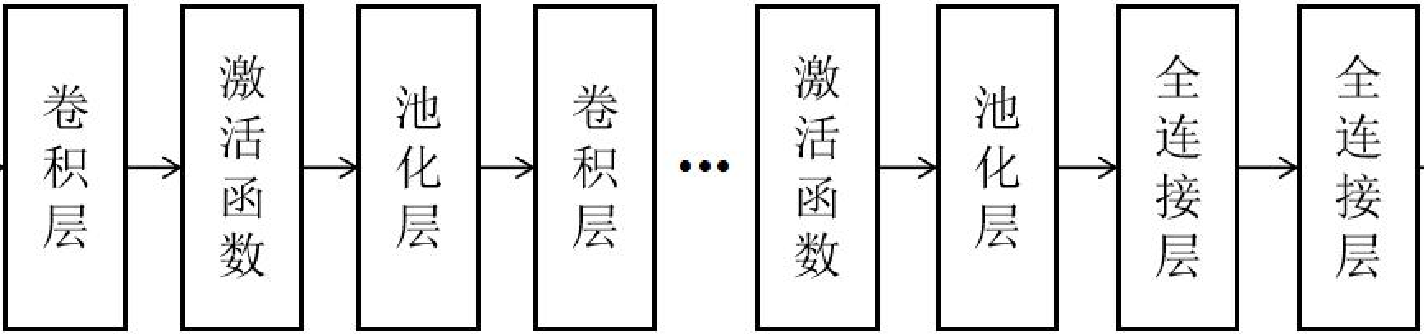
\includegraphics[width = 0.9\textwidth]{cnn.png}
    \caption{卷积神经网络常见结构}
    \label{cnn}
\end{figure}

\subsection{卷积层}
卷积层是卷积神经网络的重要组成部分之一,卷积运算实际上就是分析数学
中的一种运算方式,在卷积神经网络中最主要用到的是离散卷积运算。卷积运算的公式可以写作如式\ref{conv1}所示:
\begin{equation}
    \mathrm{s}(t)=\left(x^{*} w\right)(t)
    \label{conv1}
\end{equation}

\begin{figure}[htbp]
    \centering
    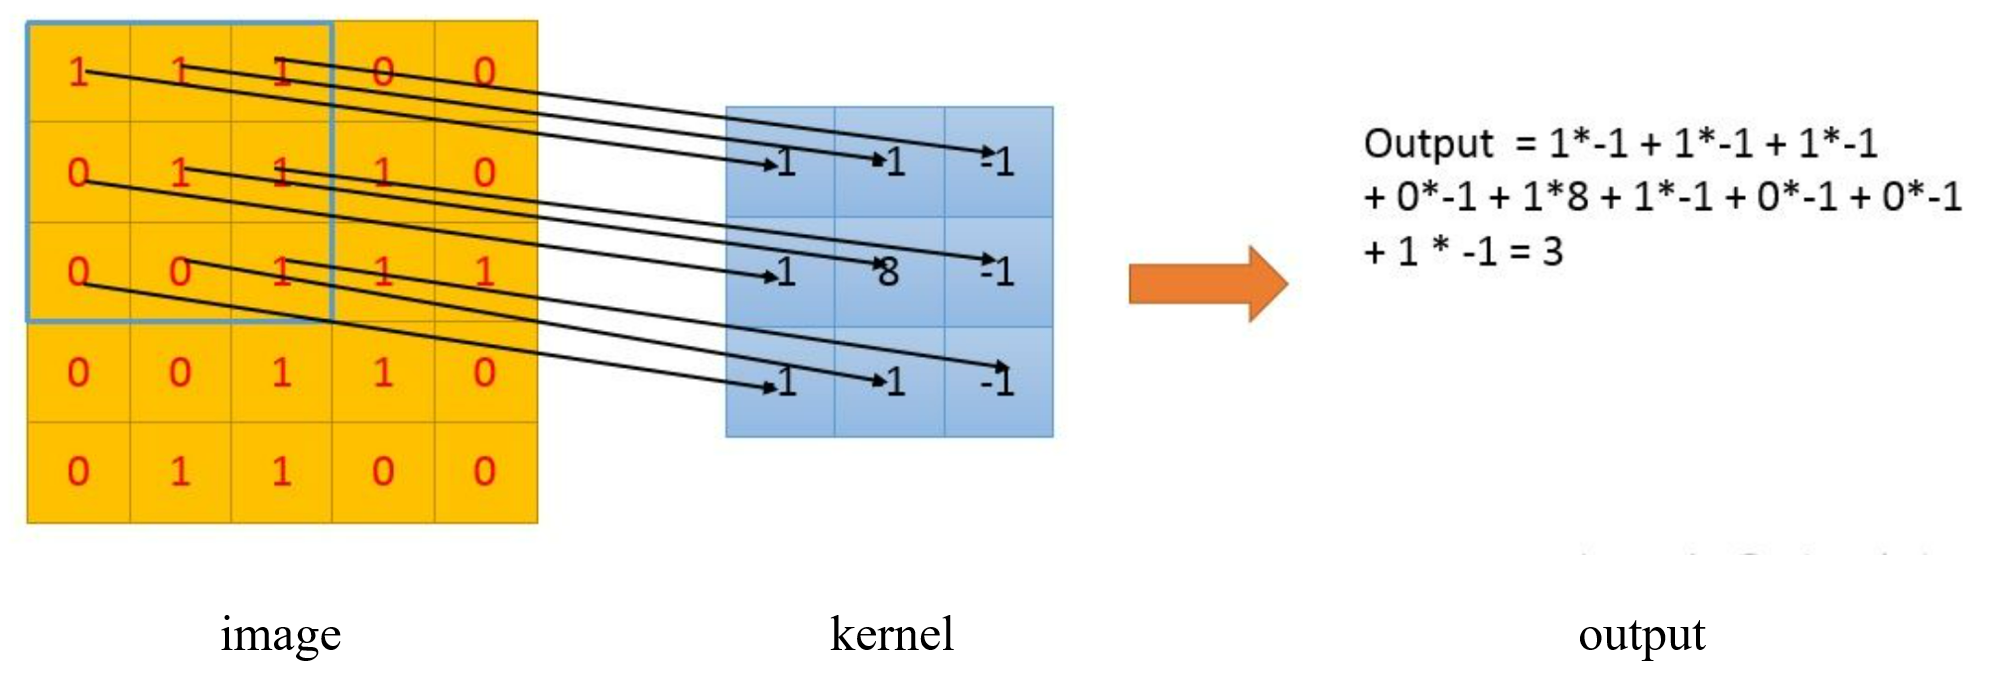
\includegraphics[width = 0.9\textwidth]{jjgc.png}
    \caption{图像卷积运算过程}
    \label{jjgc}
\end{figure}

其中$x$代表输入,$w$ 代表核函数。应用在图片上的卷积可以看做是二维矩阵
的乘法,卷积核的大小要远小于图像的大小,因此卷积可以看做是一种局部操作。
对图像的卷积过程如图\ref{jjgc}所示,
假设输入图像为$5\times5$的矩阵,卷积核的大小为
$3\times3$,卷积操作从图像左上角开始,即$(0,0)$坐标,本次卷积后的结果为卷积
核中的数值与图像对应位置的像素值逐位相乘后累加,之后卷积核以设定的步长
为移动单位从上到下从左到右的在图像上依次进行卷积,最终输出结果(在目标
检测中也称为特征图),结果的大小由式\ref{cout}决定,
\begin{equation}
    N_{\text {output }}=\frac{\left(W_{\text {input }}-F+2 P\right)}{S}+1
    \label{cout}
\end{equation}

其中$W$代表输入图像大小,

\subsection{激活函数}
激活函数的引用是为了解决网络的非线性问题,增加整个网络的表达能力,
激活函数的初衷是模拟了生物神经元特性,解决之前简单线性加权难以解决的非
线性信号拟合问题。常用的激活函数如下:

(1)Sigmoid 函数:也称 Logistic 函数,该函数的数学定义式为 2.3 所示,
\begin{equation}
    \sigma(x)=\frac{1}{\exp (-x)+1}
\end{equation}

\begin{figure}[htbp]
    \centering
    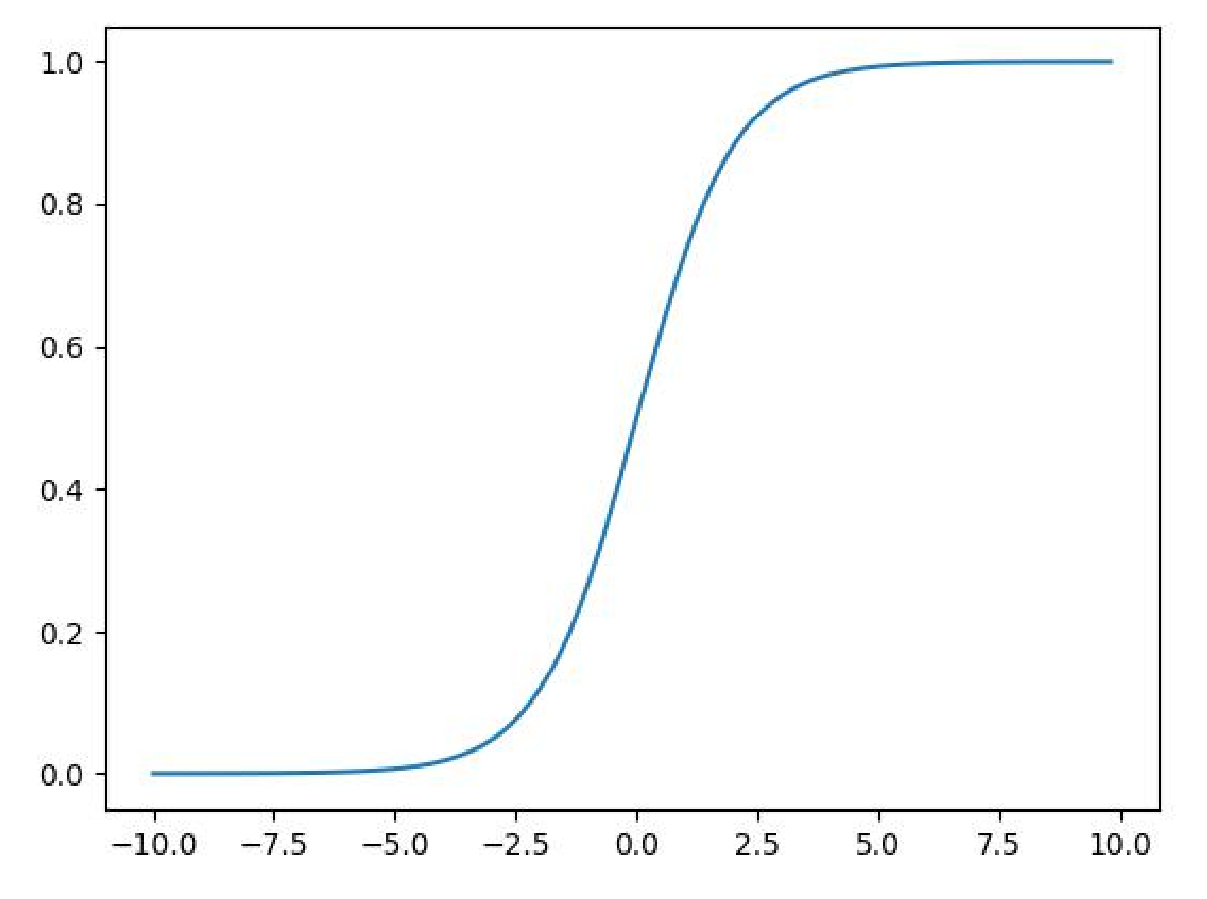
\includegraphics[width = 0.5\textwidth]{sigmoid.png}
    \caption{Sigmoid函数}
    \label{sig}
\end{figure}

\begin{figure}[htbp]
    \centering
    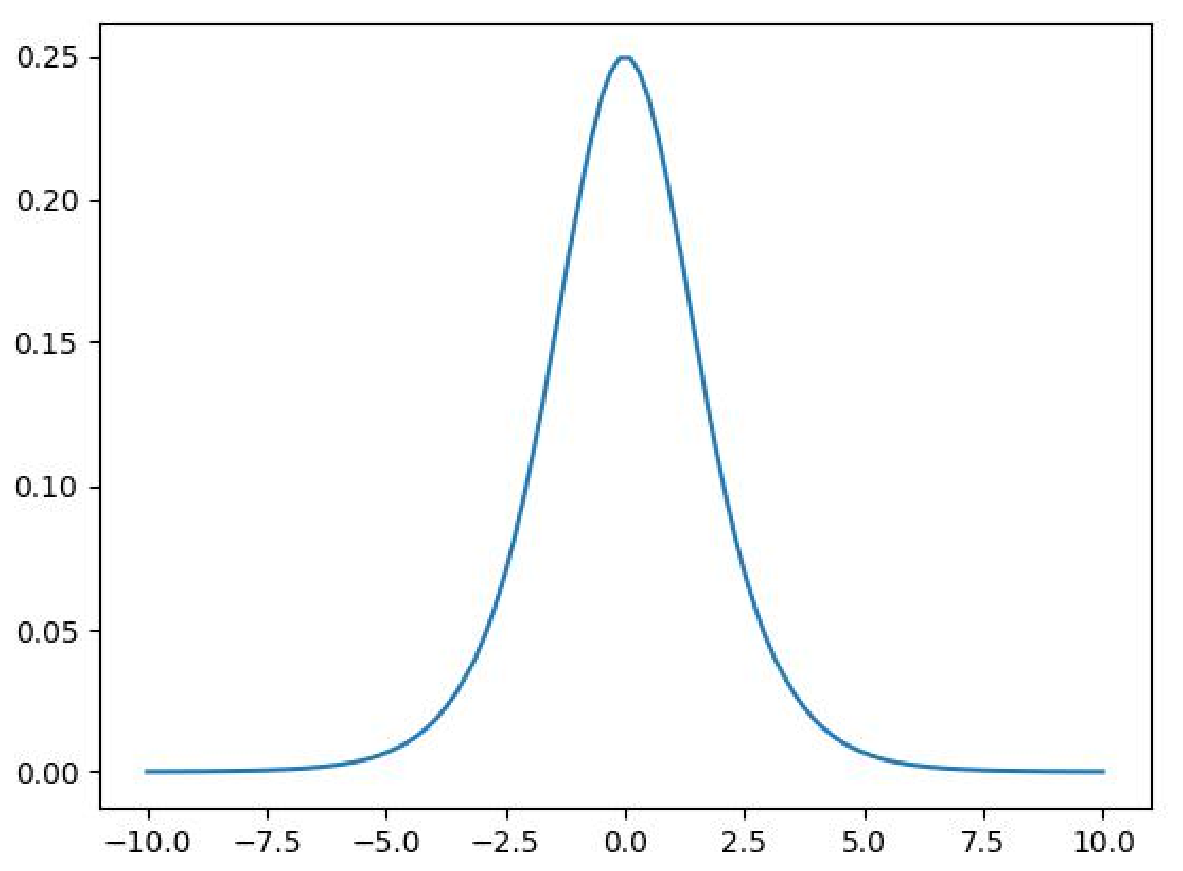
\includegraphics[width = 0.5\textwidth]{sig导数.png}
    \caption{Sigmoid导函数}
    \label{sigd}
\end{figure}

其函数图像如图\ref{sig}所示,从函数图像可以直观的看出经过 Sigmoid 函数处理后
将输出范围压缩到$[0,1]$之间,可以用于二分类,从其导数图\ref{sigd}可以看出
Sigmoid 函数易于求导,但其存在最大的局限就是当输入较大或较小时进行误差
反向传播时会出现“梯度消失”的情况,导致网络训练无法正常训练。为了避免
出现梯度消失的情况出现,后面又提出了 ReLU 函数作为替代。

(2)Tanh 函数:又叫做双曲正切激活函数,该函数是为了解决 Sigmoid 函
数均值问题提出的。该函数的数学定义式为 2.4 所示,
其函数图像如图 2.5 所示,
从函数图像可以直观的看出经过 Tanh 函数处理后的输入输出范围压缩到$[-1,1]$
之间,并且图像是以原点为中心旋转对称的,可以将 Tanh 函数看做是 Sigmoid
函数进行拉伸和下移得来的,解决了 Sigmoid 函数的 zero-centered 问题,避免随

\section{红外图像获取过程}